\section{Протоколы передачи IOT}
Интернет вещей в основном использует стандартные протоколы и сетевые технологии. Тем не менее, основные
поддерживающие технологии и протоколы Интернета вещей: RFID, NFC, Bluetooth с низким энергопотреблением,
беспроводная связь, протоколы радиосвязи с низким энергопотреблением и LTE-A. Эти технологии поддерживают
определенные сетевые функции, необходимые в системе IoT, в отличие от стандартной униформы
сеть общих систем. Расположение протоколов в разрезе модели \textit{OSI} представлено на рисунке \ref{fig:section6:transport}

\begin{figure}[h!]
    \centering
    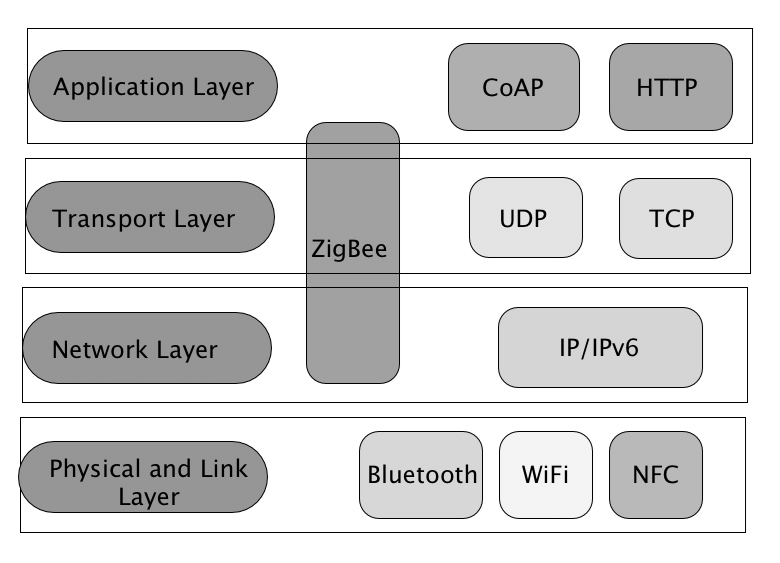
\includegraphics[scale=0.45]{transport.png}
    \caption{Протоколы передачи IOT}
    \label{fig:section6:transport}
\end{figure}

\subsection{NFC и RFID}
RFID (радиочастотная идентификация) и NFC (коммуникация ближнего радиуса действия) обеспечивают простые, энергосберегающие и универсальные возможности для идентификации и токенов доступа, начальной загрузки соединения и
платежи.
\begin{itemize}
    \item В технологии RFID используются двусторонние радиопередатчики-приемники для идентификации и отслеживания меток.
    связанные с предметами.
    \item NFC состоит из протоколов связи для электронн ых устройств, обычно мобильных устройств или карт доступа.
\end{itemize}


\subsection{Bluetooth Low Energy}
Эта технология поддерживает маломощную и длительную потребность в функции IoT при использовании стандартных протоколов обмена.

\subsection{Радиосвязь}
ZigBee, Z-Wave и Thread — это радиопротоколы для создания низкоскоростных частных сетей.
Эти технологии маломощны, но обеспечивают высокую пропускную способность в отличие от многих аналогичных вариантов. Этот
увеличивает мощность небольших локальных сетей устройств без типичных затрат.

\subsection{LTE-А}
LTE-A, или LTE Advanced обеспечивает важное обновление технологии LTE (сравнение с другими технологиями приведено на рисунке \ref{fig:section6:lte-a}), увеличивая не только
покрытия, но также уменьшая задержку и повышая пропускную способность. Это дает IoT огромное
мощности за счет расширения своего диапазона, причем наиболее важными приложениями являются транспортные средства, БПЛА,
и подобное общение.

\begin{figure}[h!]
    \centering
    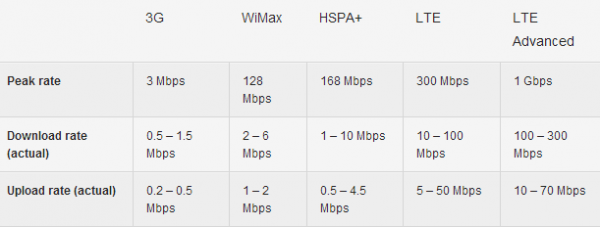
\includegraphics[scale=0.6]{lte-a.png}
    \caption{Сравнение LTA-A с существующими системами телекоммуникации}
    \label{fig:section6:lte-a}
\end{figure}